\documentclass{article}
\usepackage{graphics}
\usepackage{indentfirst}
\usepackage{amsmath}
\usepackage{algorithm}
\usepackage{algorithmic}
\usepackage{bm}
\usepackage{setspace}
\usepackage{graphicx}
\usepackage{float}
\author{Ruichen Wang}
\title{Q \& A}

\begin{document}
\maketitle
\begin{abstract}
Some basic questions worth thinking.
\end{abstract}
\noindent
\paragraph{Things you should know...}~{}

C4.5, ID3, CART, K-means, SVM, Kernel function, SMO, EM, Naive bayes, Variational inference, PageRank, Adaboost, KNN,  Linear regression, Logistic regression, LDA, PCA, Random Forest, Bagging \& stacking, Softmax, GBDT, Xgboost, LightGBM, PCA, Max-entorpy, Gradient diminishing, FM, LFM, MF, SVD, SVD++, Simhash, Max likelihood, ALS, L1 norm, L2 norm, Discriminate \& Generative model, Entorpy, Cross-entropy, KL divergence, SGD, BGD, MBGD, Adam, Newton's method, Unbiased estimator, F1 score, Recall, Prercision, AUC, ROC, Cross validation, Bias-Variance tradeoff, Loss function, Overfitting \& underfitting, DBSCAN, TF-IDF, Text rank, Word2vec, Glove, Fast-text, Collaborative Filtering, User-cf, Item-cf, Dropout, Batch norm, Maxpooling, Avg pooling, Global avg pooling, Respective field, LR normalization, Online learning, FTRL, FOBOS, RDA, Tree row \& column sampling,  ANN, Tree normalization, RNN, LSTM, GRU, CRF, RNN \& CNN, KDtree, Resnet, Seq2seq, Deep wise CNN, 1X1 kernel, SVM multi-classification, Attention, Conv complexity, Pearson correlation


\paragraph{Why L1 regulation generates sparsity? L2 regulation cause blur?}~{}

Firstly, why do we want the result matrix to be sparse?

Consider 1 million dimension, calculate the inner product between $w$ and $x$ need a lot of computation. If the $w$ can be sparse, the inner product will only be performed on the non-zero columns.

Or consider another situation, in some scenario, there are free data and many features, which is often called as \textbf{`small n, large p problem'}. If $n \ll p $, then our model will be very complex, our $w$ will be a singular matrix ($|w|=0$). In other words, \textbf{overfitting}.

One way to control overfitting is adding a regularization term to the loss function. Rigde  ($l_{2} norm$) and LASSO ($l_{1} norm$) regression are two very common regression ways.
$$J(w)=Loss(x)+\lambda ||w||_{2}^{2}$$
$$J(w)=Loss(x)+\lambda ||w||_{1}$$
Assume we use loss using MSE, the target function can also be denoted as :
$$ \mathop{\min}_{w} \frac{1}{n}||y-Xw||^{2} \quad  s.t. \lambda ||w||_{2}^{2} \leq C $$
$$ \mathop{\min}_{w} \frac{1}{n}||y-Xw||^{2} \quad  s.t. \lambda ||w||_{1} \leq C $$

Back to the problem, intuitivly, the target loss will alway intersect at the coordinate axis when using l1 norm. Imaging high dimension situation, the angles will certainly more likely to be intersected, while the ball will not.

\begin{figure}[H]
\centering
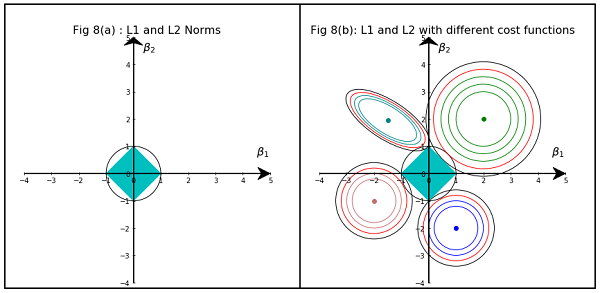
\includegraphics[width=3.5in,height=1.7in]{l1l2}
\caption{L1 and L2 norm.}
\end{figure}

For more math proof, see \textit{http://freemind.pluskid.org/machine-learning/sparsity-and-some-basics-of-l1-regularization}

\paragraph{Why L2 regulation cause blur?}~{}

In generative models, eg.VAE, L2 norm / L2 loss / MSE tend to yield blurry images. We try to explain this in probabilistic settings. In Gaussian distribution, it defines as :
$$p(x|\mu,\sigma^{2})=\frac{1}{Z}exp\left( -\frac{||\mu-x||^{2}}{2\sigma^{2}}\right)$$
$$logp(x|\mu,\sigma^{2}) \propto exp\left(-\frac{1}{2}||x_{\mu}-x||^{2}  \right)$$
As we can see, minimizing MSE, is same as maximizing the log likelihood of gaussian, we make the assumption that our $x$ comes from a gaussian.


\begin{figure}[H]
\centering
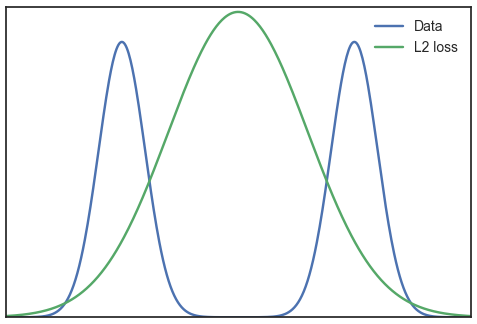
\includegraphics[width=3in,height=1.7in]{l2}
\caption{Gaussian and multinomial.}
\end{figure}

In reality, there often many hidden variables (multinomial) controls the $x$. A simple example, we have white and black dogs as dataset $x$. maximizing the likelihood will blur the two and generate gray dogs.

\paragraph{One-hot encoding for gbdt?}~{}

It is often the case that we have continuous and categorical features. One-hot encoding may produce very sparse variables. Tree based algorithm tries to increase information gain on the data it`s splitting at any given level. If the data is very sparse, the one-hot encoded feature may be ignored as they are far too sparse. 

\textit{Then how to using categorical features  in trees?} 

In xgboost \cite{DBLP:conf/kdd/ChenG16}, it treat every input as numerical, It may be helpful is the categories as small. Otherwise, it may downgrade the performance. 

In lightGBM, it said that a tree built on one-hot features tends to be unbalanced and needs to grow very deep to achieve good accuracy. It`s automaticly provide a optimal solution $O(k*logk)$ to find the best optimal partition. This often performs better than one-hot encoding. 

For more info, see lightgbm api.

\paragraph{xgboost, lightGBM, gbdt, GBM?}~{}

Gradient tree boosting is also known as gradient boosting machine (GBM) or gradient boosted regression tree (GBRT). 

\textbf{xgboost} using taylor expansion to approximate the objective function. Regularization is defined as number of leafs plus l2 norm of leaf values.
 
\begin{figure}[H]
\centering
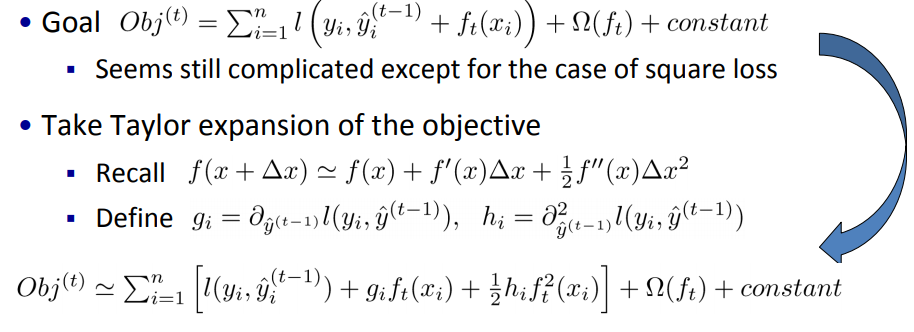
\includegraphics[width=4in,height=1.5in]{taylor}
\caption{}
\end{figure}

for detail see pdf in ml papers basis.

\textbf{lightgbm} choose the leaf with max delta loss to grow(leaf wise, best first), while most tree grow by level wise. Using max depth to control overfitting.

\paragraph{bagging vs boosting vs stacking}~{}

bagging Bootstrap Aggregating 
\paragraph{xgb rf lr difference}~{}
\paragraph{user-cf item-cf difference and application scenarios}~{}
\paragraph{svm vs lr}~{}
\paragraph{lstm vs gru}~{}

\bibliographystyle{plain}
\bibliography{ref}
\end{document}

























